\section{Node.js}
\label{sec:node}
\begin{figure}
	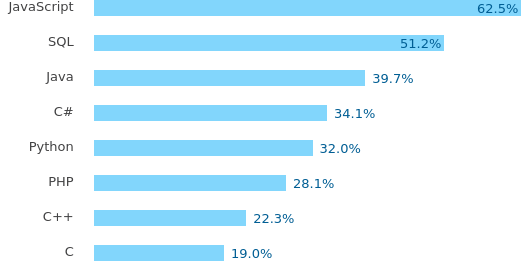
\includegraphics[width=.5\textwidth]{fig/languages}
	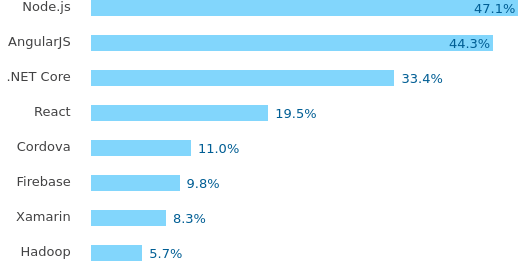
\includegraphics[width=.5\textwidth]{fig/frameworks}
	\caption{Stack Overflow Developer Survey 2017, \url{https://insights.stackoverflow.com/survey/2017}. Most used programming languages (on the left) and frameworks (on the right).}
	\label{fig:popularity}
\end{figure}
%\paragraph{JavaScript}
%According to a survey conducted among developers all over the world by the Stack Overflow website, JavaScript is currently the most popular programming language (\Cref{fig:popularity}), having been a de facto standard for client-side web development for a long time.

%JavaScript is a high-level, dynamic scripting language supporting multiple paradigms: imperative, object-oriented, event-driven and functional programming.
%Standardized as EcmaScript \cite{EcmaScript}, the language is under active development and new features are constantly added, with the latest stable version released in June 2017.

\paragraph{Node.js}
In 2009 Node.js\footnote{\url{https://nodejs.org/}} was released, and since then its popularity quickly raised to the point that it now appears to be the single most used framework, according to Stack Overflow Developer Survey 2017 (\Cref{fig:popularity}).
Node.js is a JavaScript runtime environment expressly devised for running JavaScript code outside web browsers, thus giving developers the opportunity to use the language to write server-side code as well.

Node.js is based on Chrome V8, a highly optimized JavaScript engine developed for the Google Chrome web browser. 
Furthermore, developers can count on a huge package ecosystem\footnote{\url{https://www.npmjs.com/}} with a repository of hundreds of thousand modules that can be reused.
More recently, Node.js has become relevant for the Internet of Things as well, both because of the availability of packages for device management and its asynchronous model, which is well suited for distributed environments.
Node-RED\footnote{\url{https://nodered.org/}} is a tool based on Node.js to support flow-based programming for the Internet of Things to
connect together devices at the edge of the network.

\paragraph{Asynchronous Computation}
%The execution model of Node.js is quite different from most of other environments.
In Node.js, connection to databases, HTTP requests, access to the file system and every other I/O intensive operation is by default \emph{asynchronous}, meaning the actual execution is postponed until a later time, and the program can go on without waiting for completion.
Computations needing the results of I/O operations are modeled by \emph{callbacks}: when an asynchronous function is invoked, another function (the callback) is given as an additional argument, and it will be executed once the results will be available.

\Cref{lst:async} shows the different programming patterns using synchronous and asynchronous calls.
On the left, the program is blocked until the result of \lstinline{syncIO} is returned, and then it is passed to function \lstinline{use}.
On the right, \lstinline{asyncIO} \emph{immediately returns} and the I/O operation is scheduled for execution together with the callback \lstinline{use}; when the result will be available, the callback will be executed receiving such result as an argument.
Node.js heavily takes advantage of the right pattern (for the sake of brevity, error handling is ignored in the example).

\begin{figure}[h]
\begin{minipage}{.5\textwidth}
\begin{lstlisting}
	function use(data) { ... }
	let res = syncIO(...);
	use(res);
\end{lstlisting}
\end{minipage}
\begin{minipage}{.5\textwidth}
	\begin{lstlisting}
	function use(data) { ... }
	asyncIO(..., use);
	\end{lstlisting}
\end{minipage}
\caption{Difference between synchronous and asynchronous I/O.}
\label{lst:async}
\end{figure}

\paragraph{Event Loop}
The core of Node.js is the \emph{event loop}, represented in \Cref{fig:eventloop}.
Asynchronous requests are processed from a simple loop, and the corresponding I/O intensive operations are scheduled for execution together with their callbacks.
The event loop is run after the whole Node.js script is evaluated.

\begin{figure}[h]
	\centering
	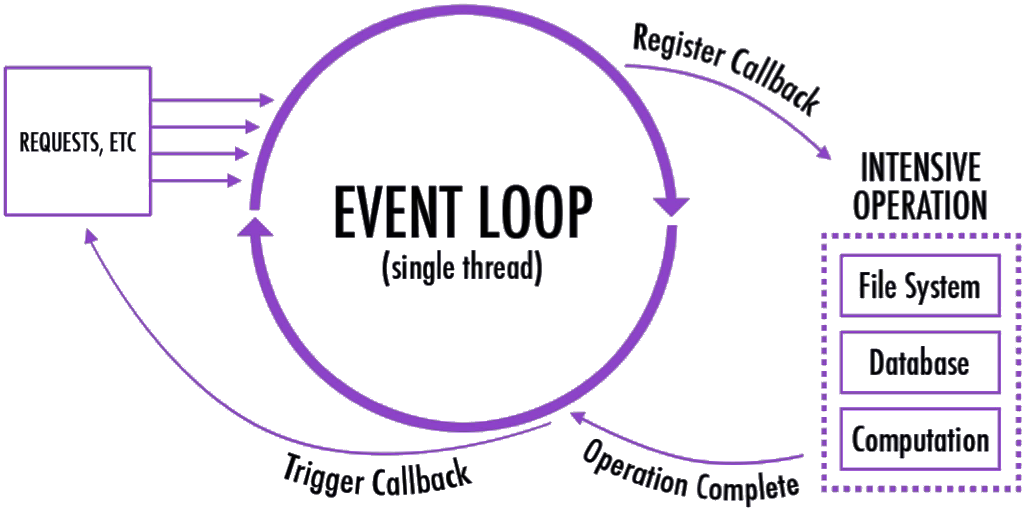
\includegraphics[width=.7\textwidth]{fig/event-loop}
	\caption{Node.js execution model representation based on the event loop.}
	\label{fig:eventloop}
\end{figure}

Note that callbacks themselves can make more asynchronous requests to the event loop, and those requests will receive callbacks, and so on\dots{}
Indeed, in real programs callbacks and I/O operations are usually nested into each other as a synchronization mechanism, making it hard to understand (and debug) the code.

Even if it may seem counterintuitive at first, this execution model based on asynchronous I/O and the event loop scales very well to a lot of concurrent operations, without the need for the programmer to explicitly deal with concurrency and parallelism \cite{Nodejs10,NodejsPerformance14}.
At the system level, different I/O operations can be executed in parallel.
